
\section{Programación de la serie de Fourier en lenguaje C}\label{programaciuxf3n-de-la-serie-de-fourier-en-lenguaje-c}

\subsection{\texorpdfstring{Implementación de código }{Implementación de código }}\label{implementaciuxf3n-de-cuxf3digo}

\begin{enumerate} \def\labelenumi{\arabic{enumi}.} \item   Se incluyen las bibliotecas necesarias para su funcionamiento y se   define el valor de PI y las constantes necesarias, finalmente \end{enumerate}

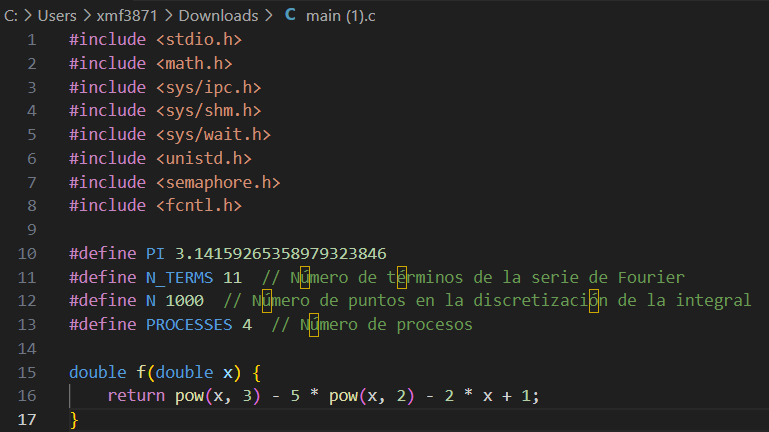
\includegraphics[width=5.55729in,height=3.12944in]{media/image18.png}

Imagen 5. Código

\begin{enumerate} \def\labelenumi{\arabic{enumi}.} \setcounter{enumi}{1} \item   La función \emph{calculate coefficients} se encarga de calcular los   coeficientes de la serie de Fourier para un rango de términos n   específico. Utiliza una técnica de sincronización con semáforos para   garantizar que cada proceso realice sus cálculos de manera ordenada. \end{enumerate}

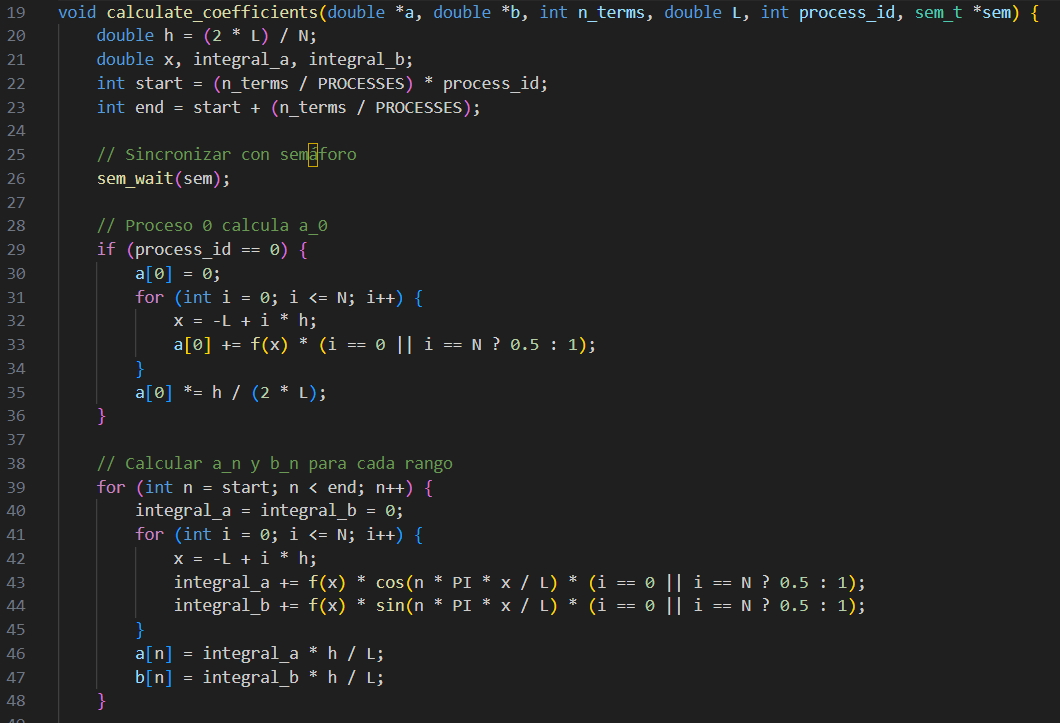
\includegraphics[width=5.64741in,height=3.85562in]{media/image39.png}

Imagen 6. Función calculate coefficients

\begin{enumerate} \def\labelenumi{\arabic{enumi}.} \setcounter{enumi}{2} \item   La función \emph{fourier\_approximation} calcula la aproximación de la   función original utilizando los coeficientes de la serie de Fourier. \end{enumerate}

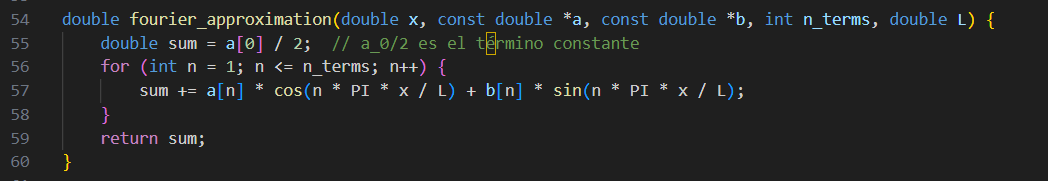
\includegraphics[width=6.26772in,height=1.08333in]{media/image11.png}

Imagen 7. Función fourier approximation

\begin{enumerate} \def\labelenumi{\arabic{enumi}.} \setcounter{enumi}{3} \item   La función \emph{export\_to\_csv} exporta los resultados a un archivo   CSV que contiene los valores de x, la función original y y la   aproximación de la serie de Fourier y\_fourier. \end{enumerate}

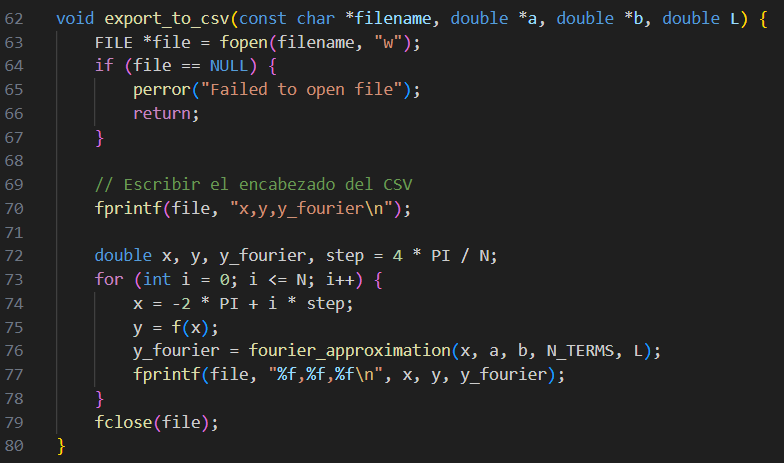
\includegraphics[width=5.02604in,height=2.61756in]{media/image50.png}

Imagen 8. Función export\_to\_csv

\begin{enumerate} \def\labelenumi{\arabic{enumi}.} \setcounter{enumi}{4} \item   En la función main, se crea un segmento de memoria compartida para   almacenar los coeficientes a y b, se crea un semáforo para la   sincronización entre procesos y se generan varios procesos hijos para   calcular los coeficientes de la serie de Fourier en paralelo. Después   de que todos los procesos hayan terminado de calcular los   coeficientes, se exportan los resultados a un archivo CSV y se liberan   los recursos utilizados. \end{enumerate}

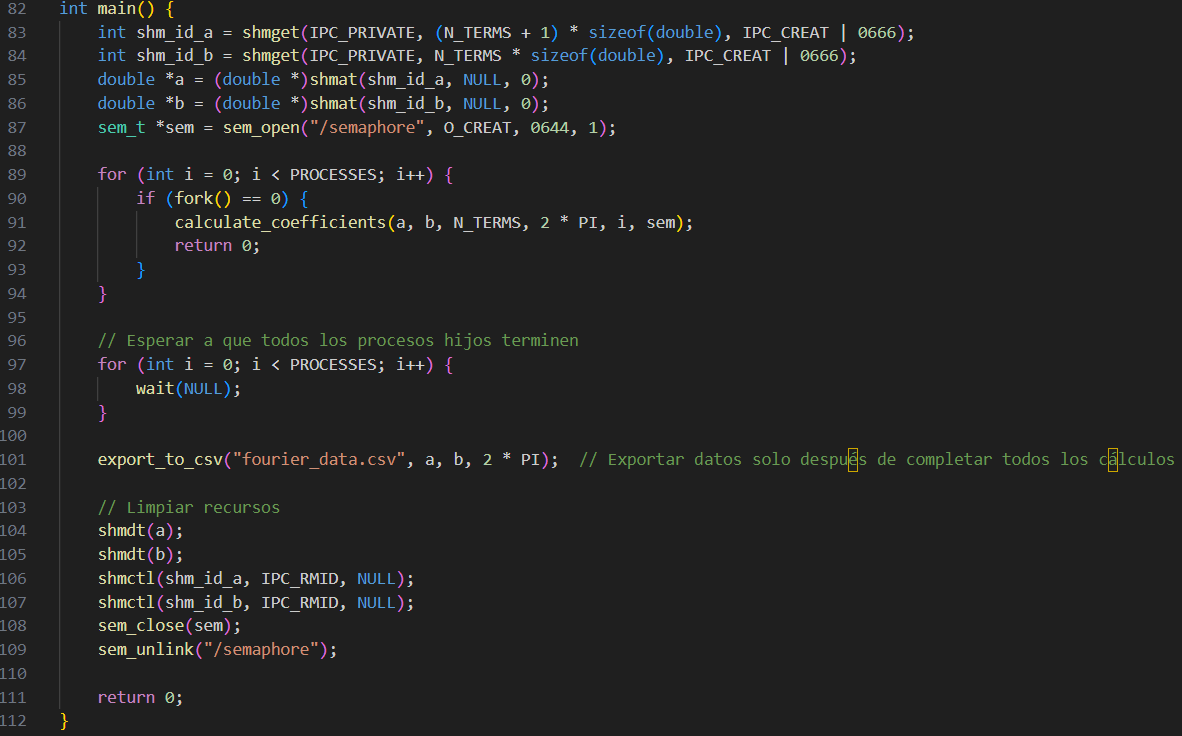
\includegraphics[width=6.26772in,height=3.90278in]{media/image7.png}

Imagen 9. Función main

\subsection{\texorpdfstring{Ejecución del código }{Ejecución del código }}\label{ejecuciuxf3n-del-cuxf3digo}

\begin{enumerate} \def\labelenumi{\arabic{enumi}.} \item   Ejecución de código en linux \end{enumerate}

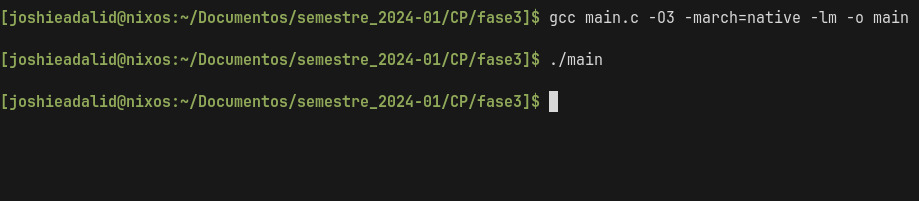
\includegraphics[width=6.26772in,height=1.375in]{media/image29.png}

Imagen 10. Ejecución en Linux

\begin{enumerate} \def\labelenumi{\arabic{enumi}.} \setcounter{enumi}{1} \item   Visualización del archivo generado. Para cada x, su evaluación el   función a aproximar, y su aproximación de la serie de Fourier \end{enumerate}

\begin{quote} 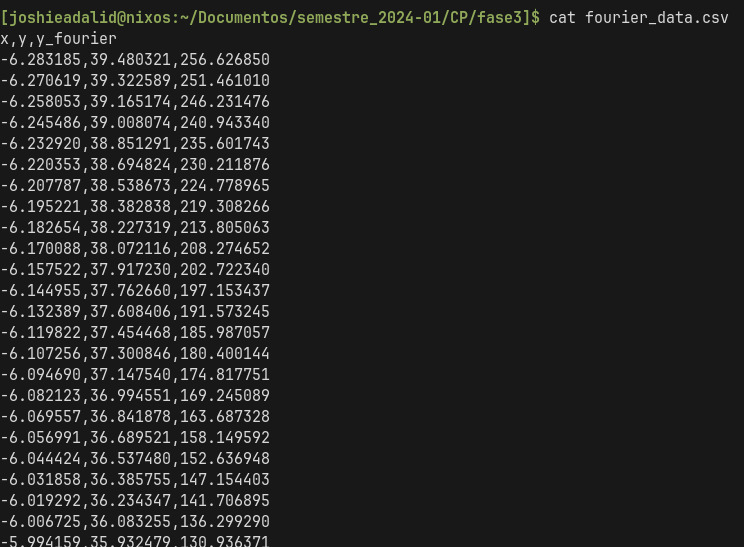
\includegraphics[width=5.16146in,height=3.79822in]{media/image37.png} \end{quote}

Imagen 11. Aproximación para la serie de Fourier

\begin{quote} 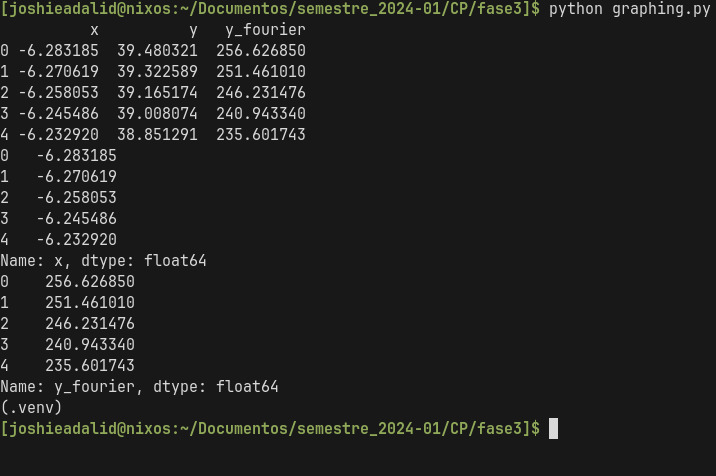
\includegraphics[width=5.16146in,height=3.42309in]{media/image25.png} \end{quote}

Imagen 12. Aproximación para la serie de Fourier

\begin{enumerate} \def\labelenumi{\arabic{enumi}.} \setcounter{enumi}{2} \item   Gráfica generada \end{enumerate}

\begin{quote} 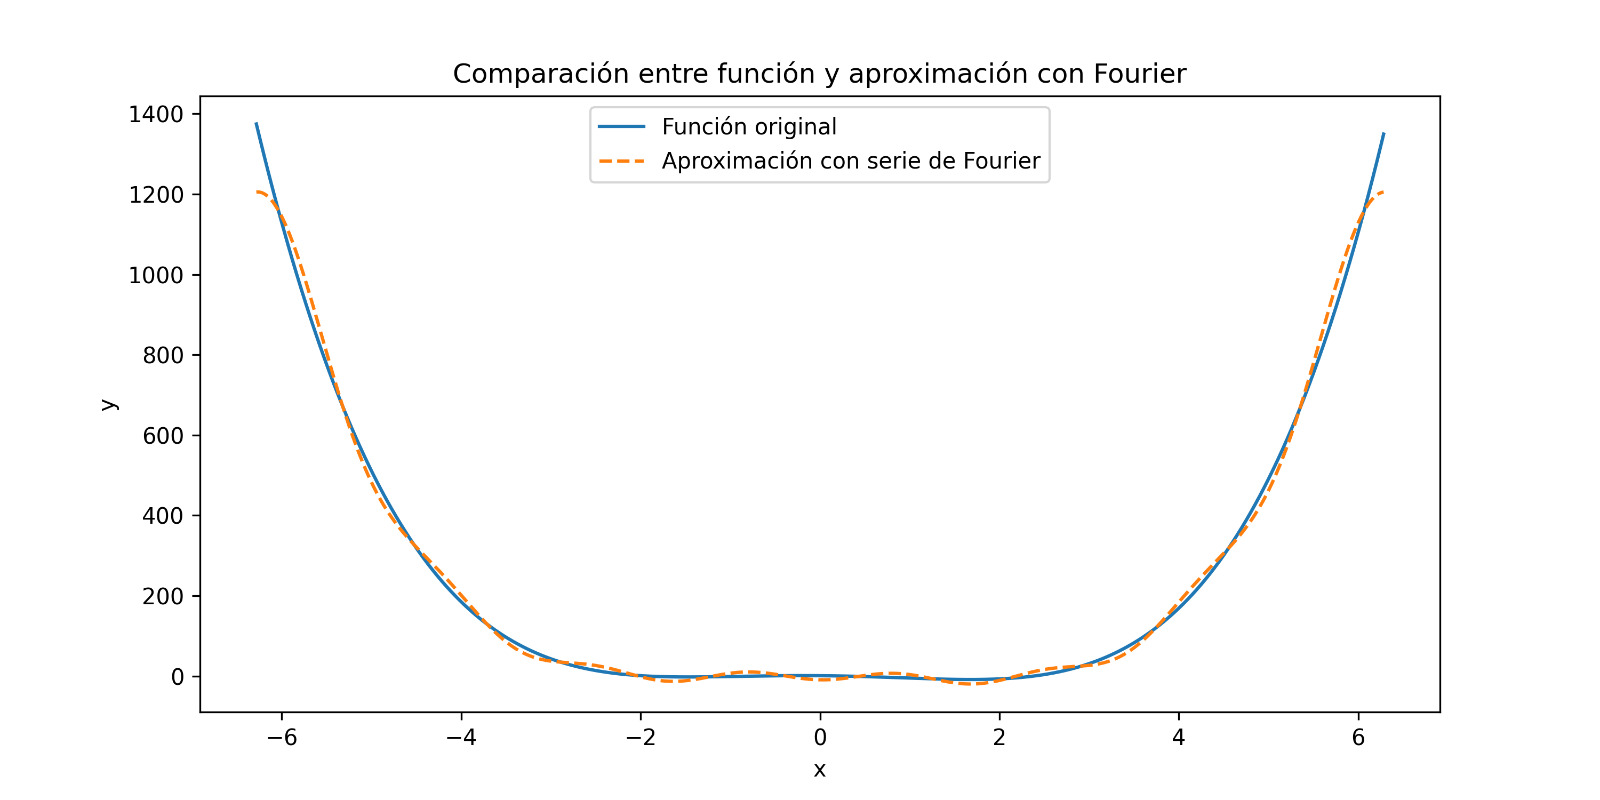
\includegraphics[width=6.26772in,height=3.13889in]{media/image12.png} \end{quote}

Figura 4. Gráfica original y aproximación de fourier en C

\subsection{Implementación de código con hilos}\label{implementaciuxf3n-de-cuxf3digo-con-hilos}

En este apartado se mostrará y explicará el código implementado ahora con hilos en lugar de memoria compartida y semáforos.

\begin{enumerate} \def\labelenumi{\arabic{enumi}.} \item   En primer lugar, se incluyen las bibliotecas necesarias para utilizar   las funciones basicas y las funciones de hilos como se muestran en la   imagen 13, así como definir unas constantes que nos ayudaran a   ejecutar el programa con hilos \end{enumerate}

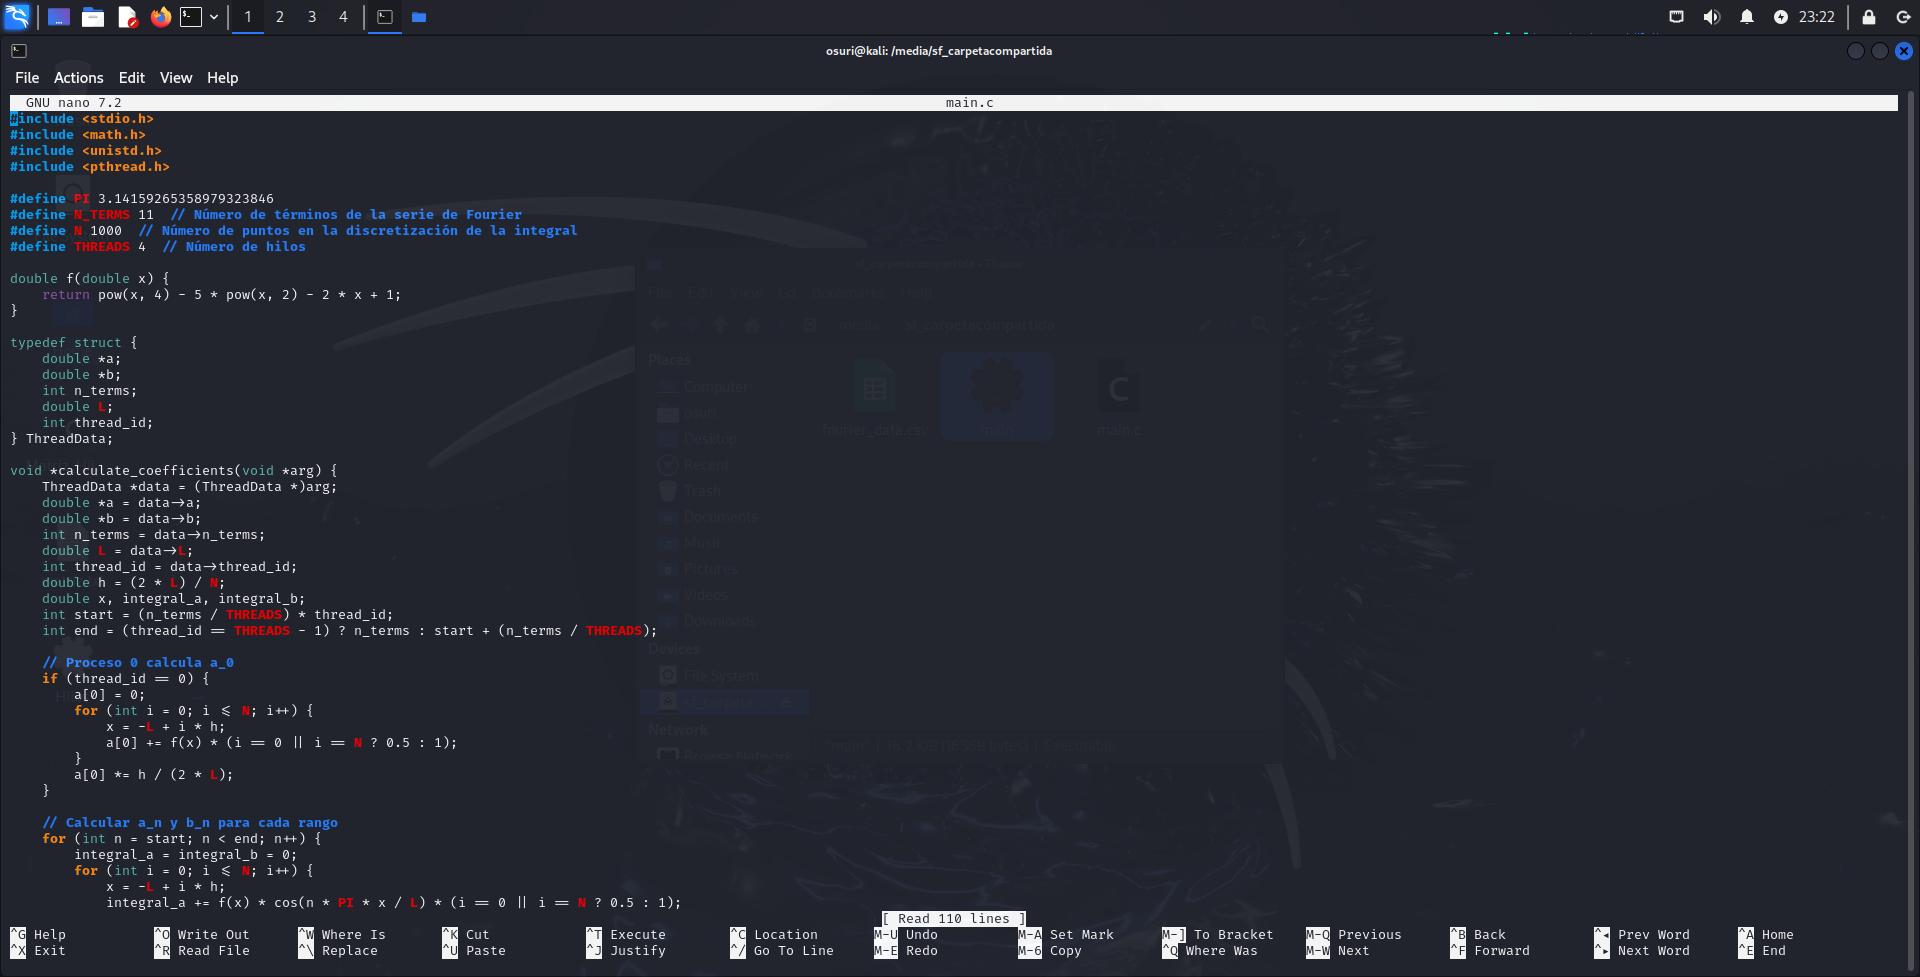
\includegraphics[width=4.53385in,height=1.24967in]{media/image4.png}

Imagen 13. Código 1. Fuente: Autoría propia

\begin{enumerate} \def\labelenumi{\arabic{enumi}.} \setcounter{enumi}{1} \item   En la imagen 14 se define la estructura básica de la serie original y   se crea la estructura de un hilo para que tenga los datos de la   ecuación de la serie, así como los valores que debe de calcular, para   almacenar múltiples tipos de datos y no entre en conflicto \end{enumerate}

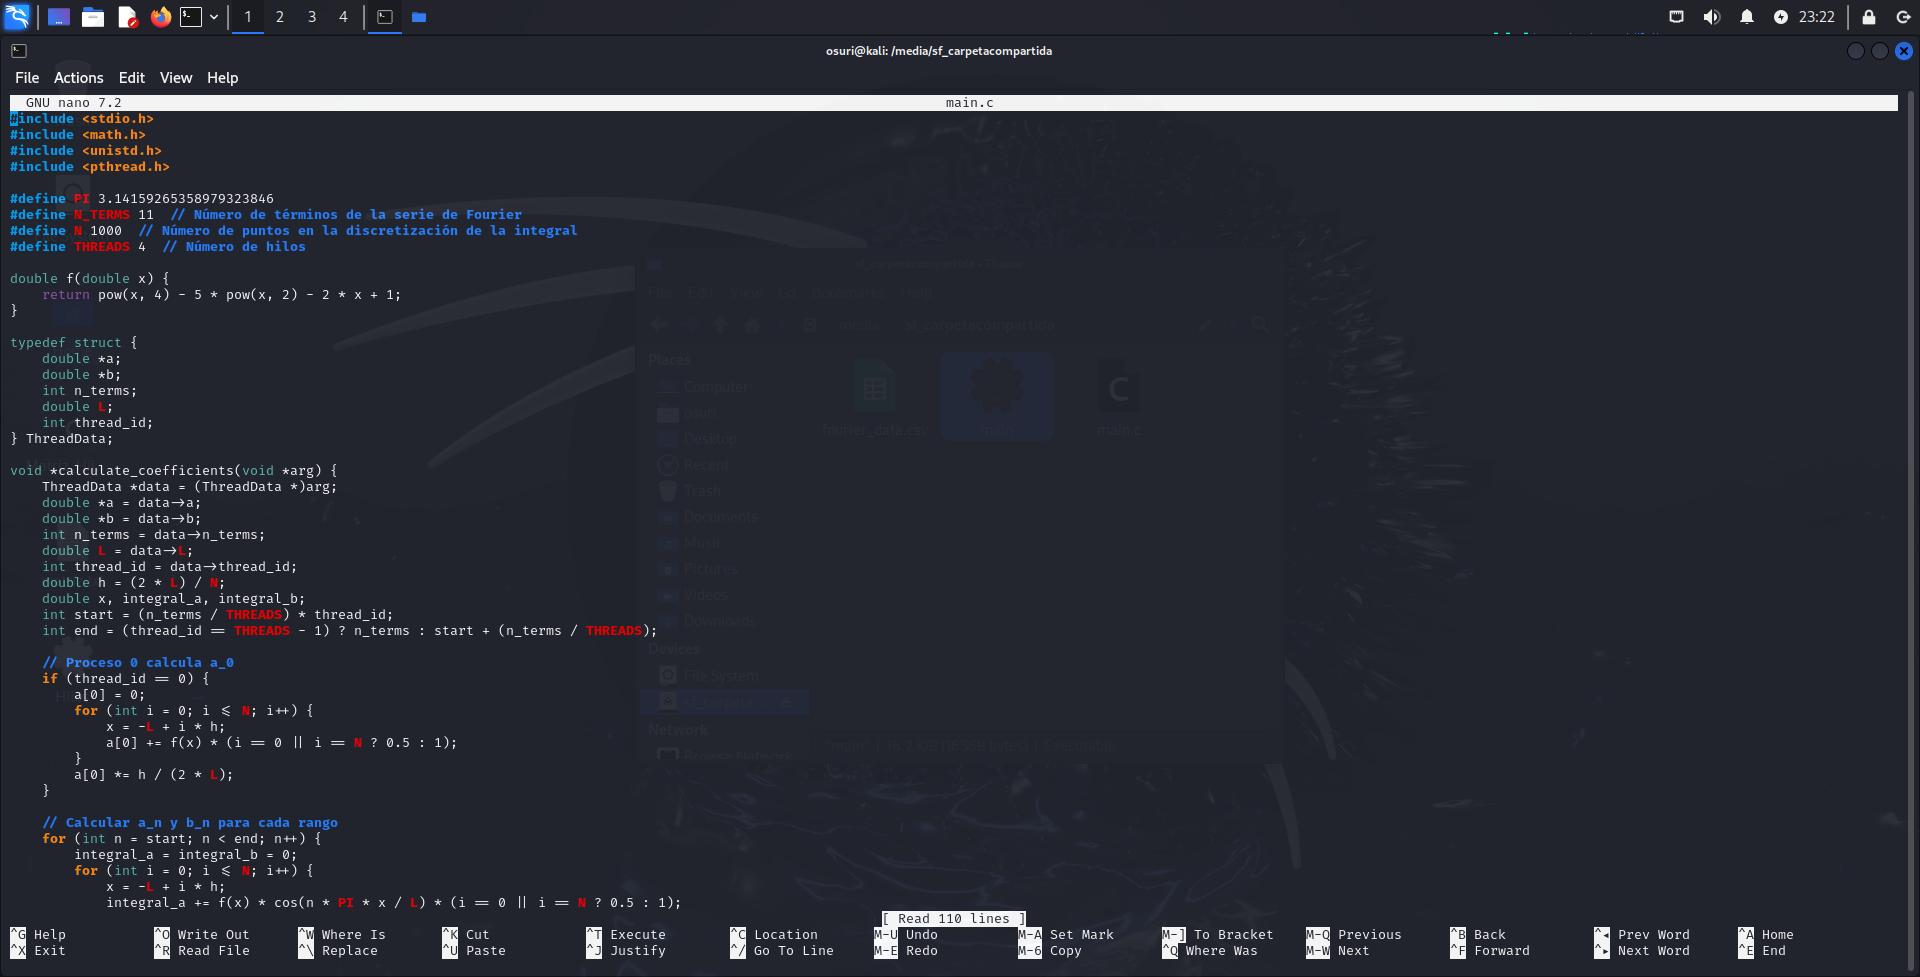
\includegraphics[width=3.15in,height=1.54172in]{media/image4.png}

Imagen 14. Código 2. Fuente: Autoría propia

\begin{enumerate} \def\labelenumi{\arabic{enumi}.} \setcounter{enumi}{2} \item   En la imagen 15, se define una función para resolver la serie de   fourier por medio de hilos, se divide la información para que pueda   ser ejecutada miles de veces, y se crean los hilos separados para   resolver los cálculos, se pone separado el cálculo de a0 porque sólo   se calcula una vez, mientras que an y bn deben ser calculados tantas   veces como ``n'' existan. \end{enumerate}

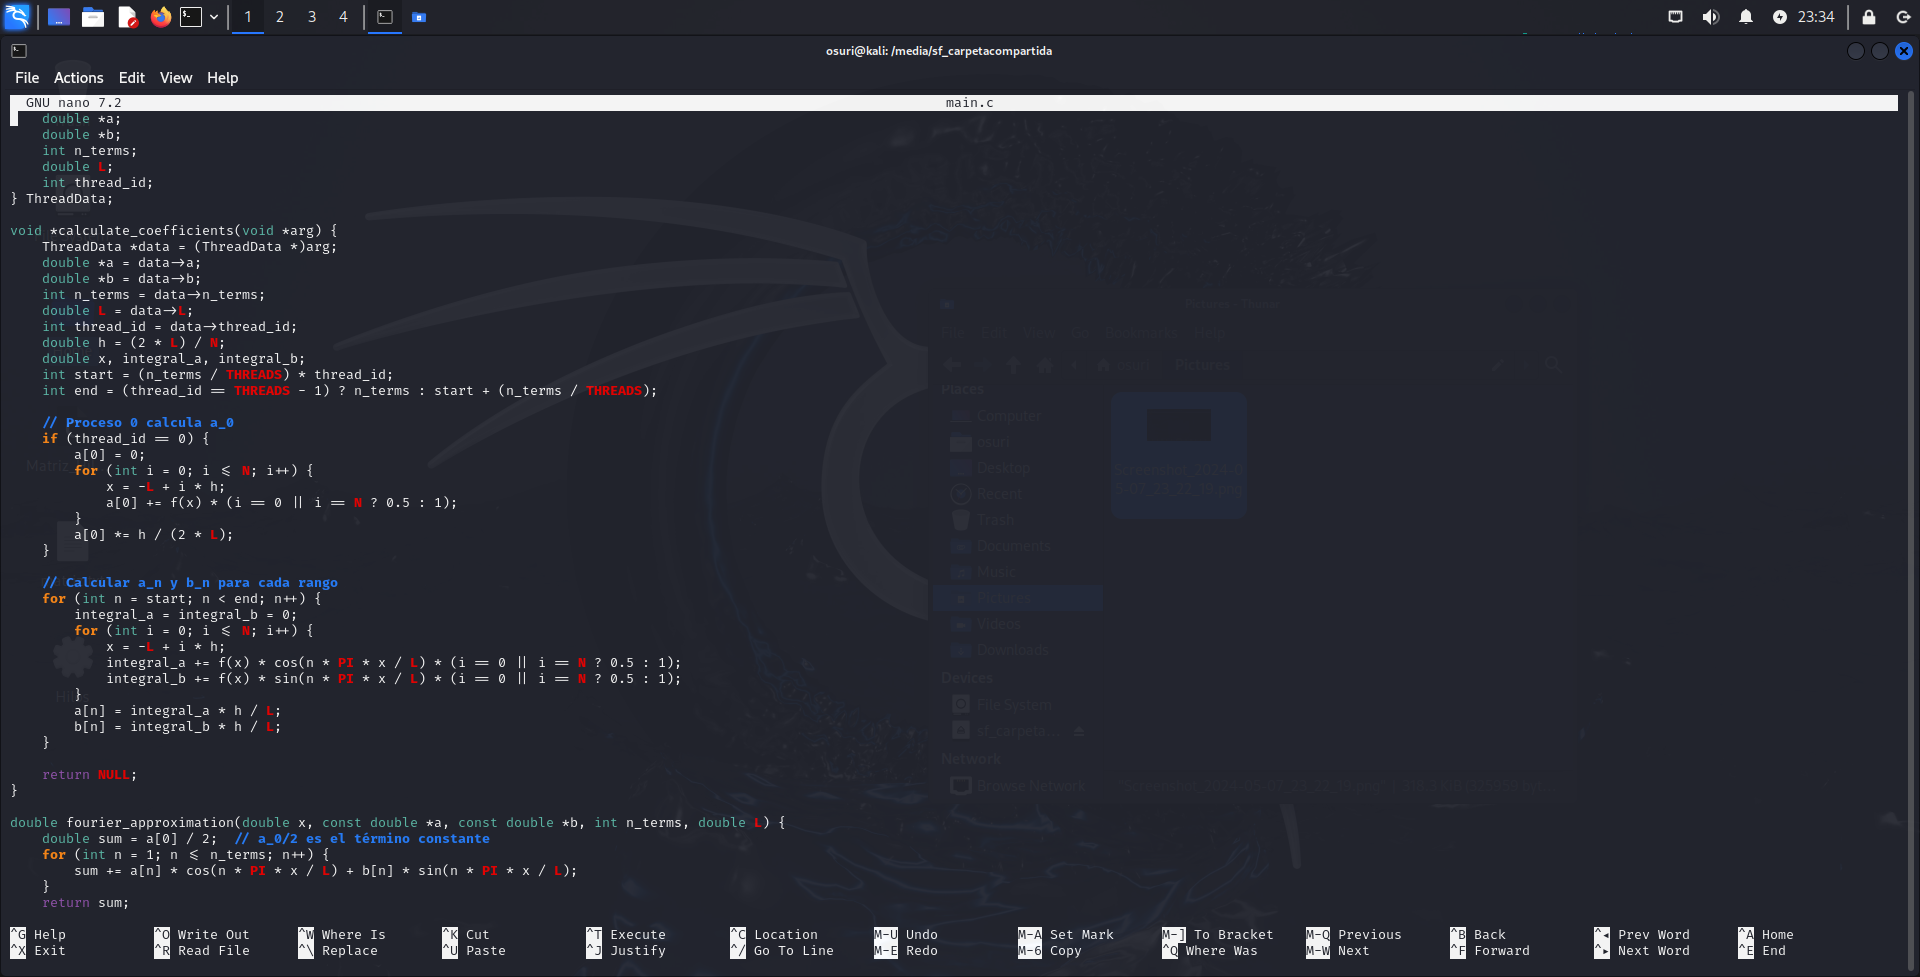
\includegraphics[width=3.00416in,height=2.52623in]{media/image17.png}

Imagen 15. Código 3. Fuente: Autoría propia

\begin{enumerate} \def\labelenumi{\arabic{enumi}.} \setcounter{enumi}{3} \item   En la imagen 16 se crea una función de aproximación con la serie   original para comparar los valores. \end{enumerate}

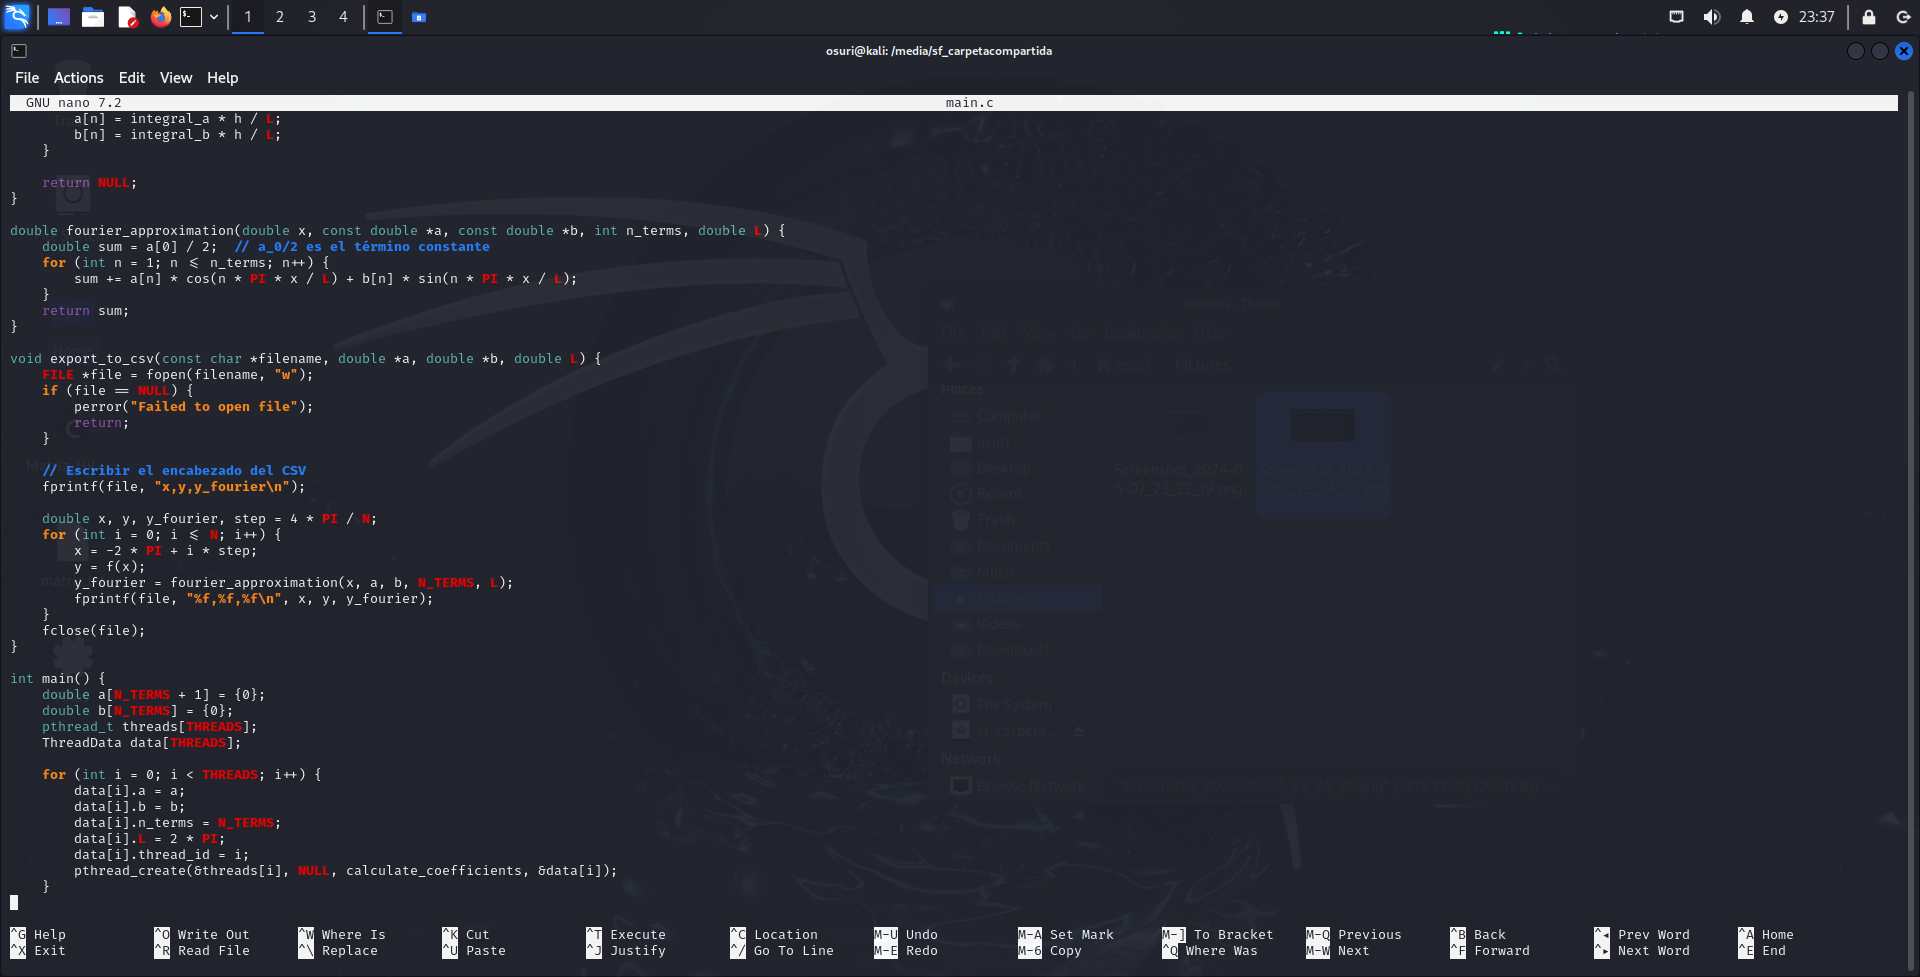
\includegraphics[width=4.31145in,height=0.71292in]{media/image27.png}

Imagen 16. Código 4. Fuente: Autoría propia

\begin{enumerate} \def\labelenumi{\arabic{enumi}.} \setcounter{enumi}{4} \item   En la imagen 17, se crea la función para exportar los cálculos   exitosos a un archivo csv para poder guardarlos y consultarlos. \end{enumerate}

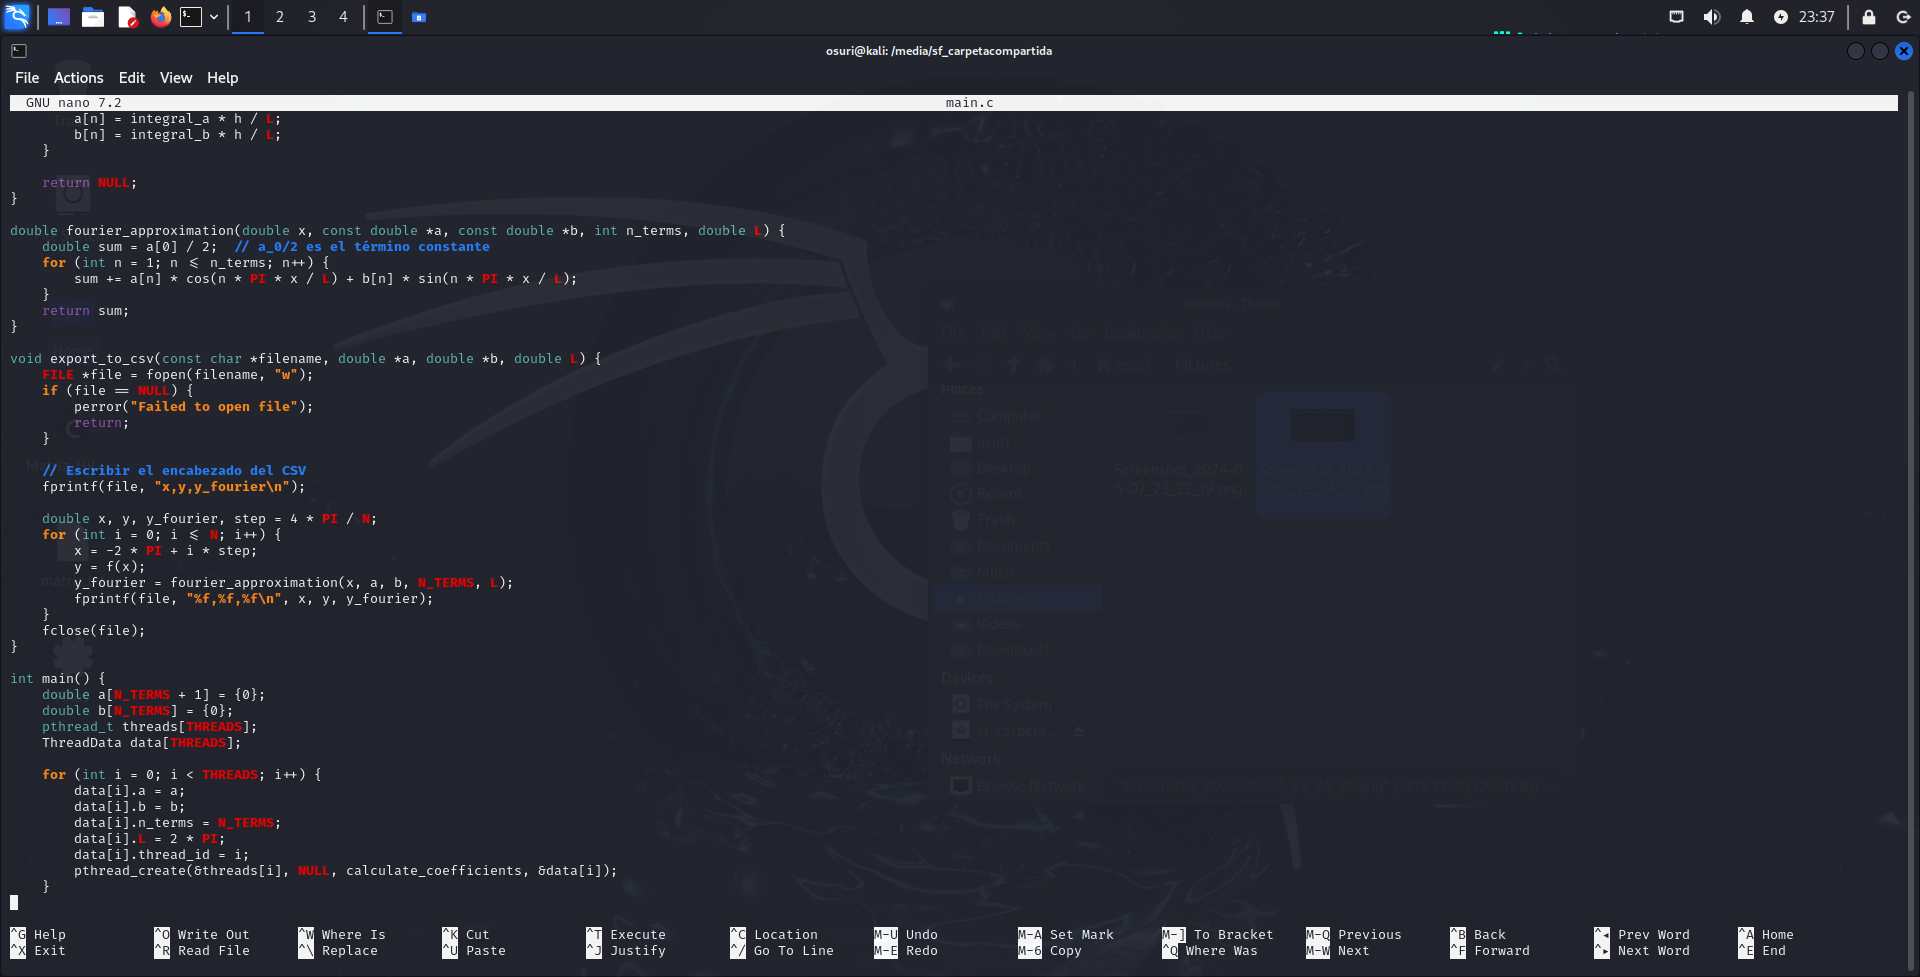
\includegraphics[width=4.19531in,height=2.2036in]{media/image27.png}

Imagen 17. Código 5. Fuente: Autoría propia

\begin{enumerate} \def\labelenumi{\arabic{enumi}.} \setcounter{enumi}{5} \item   En la imagen 18, se puede observar el programa main, donde se ejecuta   el proceso principal, se crean los hilos de acuerdo a la cantidad de   veces que se ejecutará la secuencia, en este caso 1000, se utilizará   la estructura del hilo definida con anterioridad para ejecutar los   hilos, y finalmente se utilizara la función para exportar a csv para   guardar los datos. \end{enumerate}

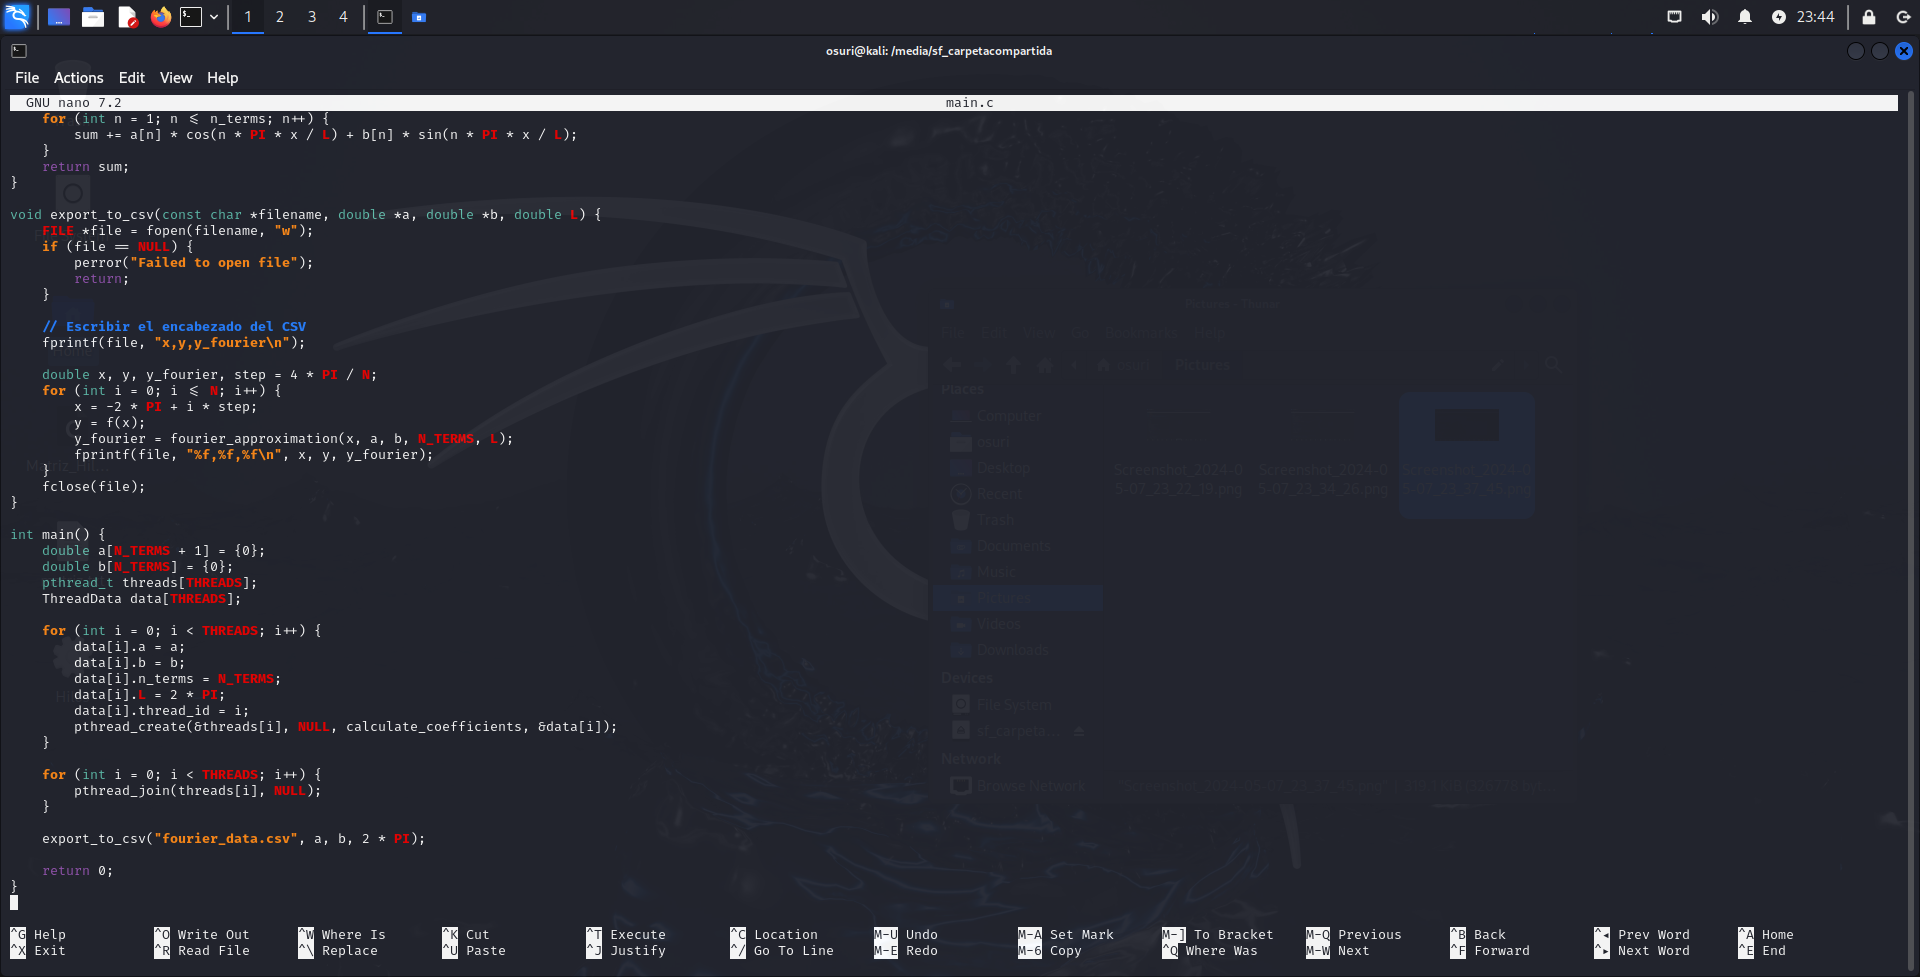
\includegraphics[width=3.82031in,height=2.4068in]{media/image5.png}

Imagen 18. Código 6. Fuente: Autoría propia

\subsection{Ejecución del código con hilos}\label{ejecuciuxf3n-del-cuxf3digo-con-hilos}

\begin{enumerate} \def\labelenumi{\arabic{enumi}.} \item   Compilación y ejecución (ver imagen 19). \end{enumerate}

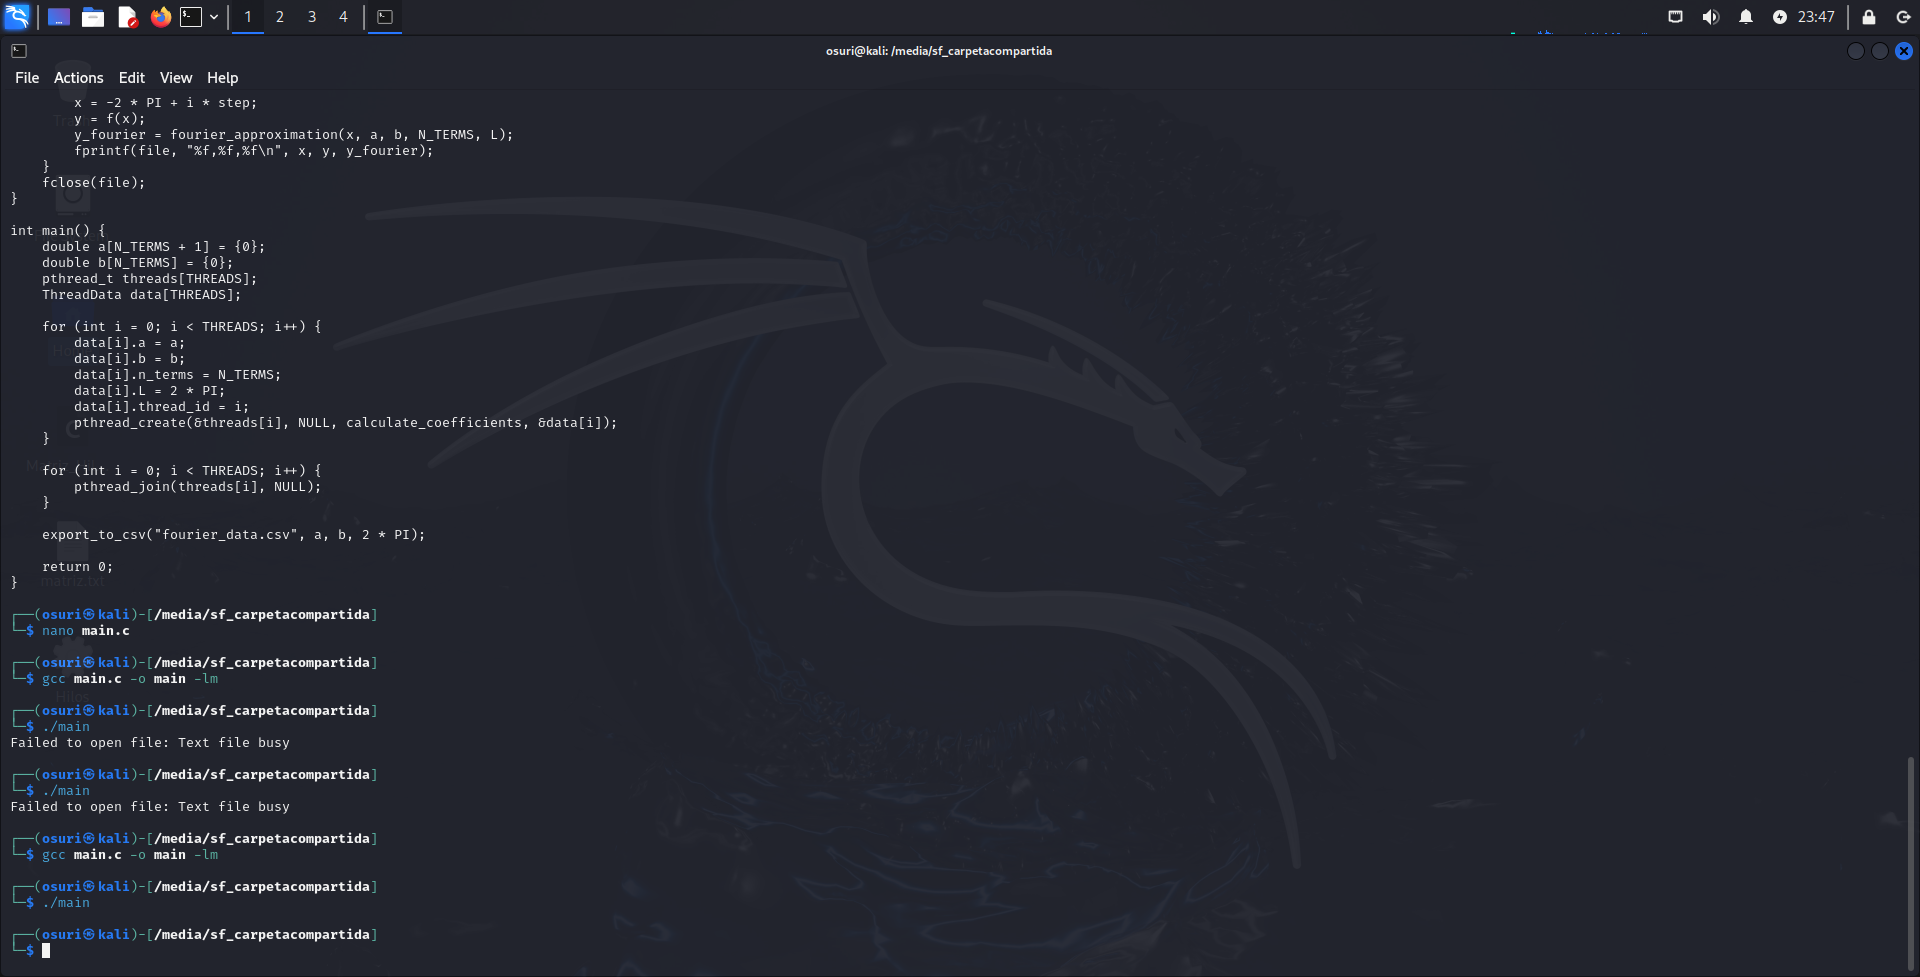
\includegraphics[width=3.46875in,height=0.8384in]{media/image36.png}

Imagen 19. Compilación y ejecución. Fuente: Autoría propia

\begin{enumerate} \def\labelenumi{\arabic{enumi}.} \setcounter{enumi}{1} \item   Visualización menor de datos, solo se utilizan ciertos datos para no   saturar el documento (ver imagen 20). \end{enumerate}

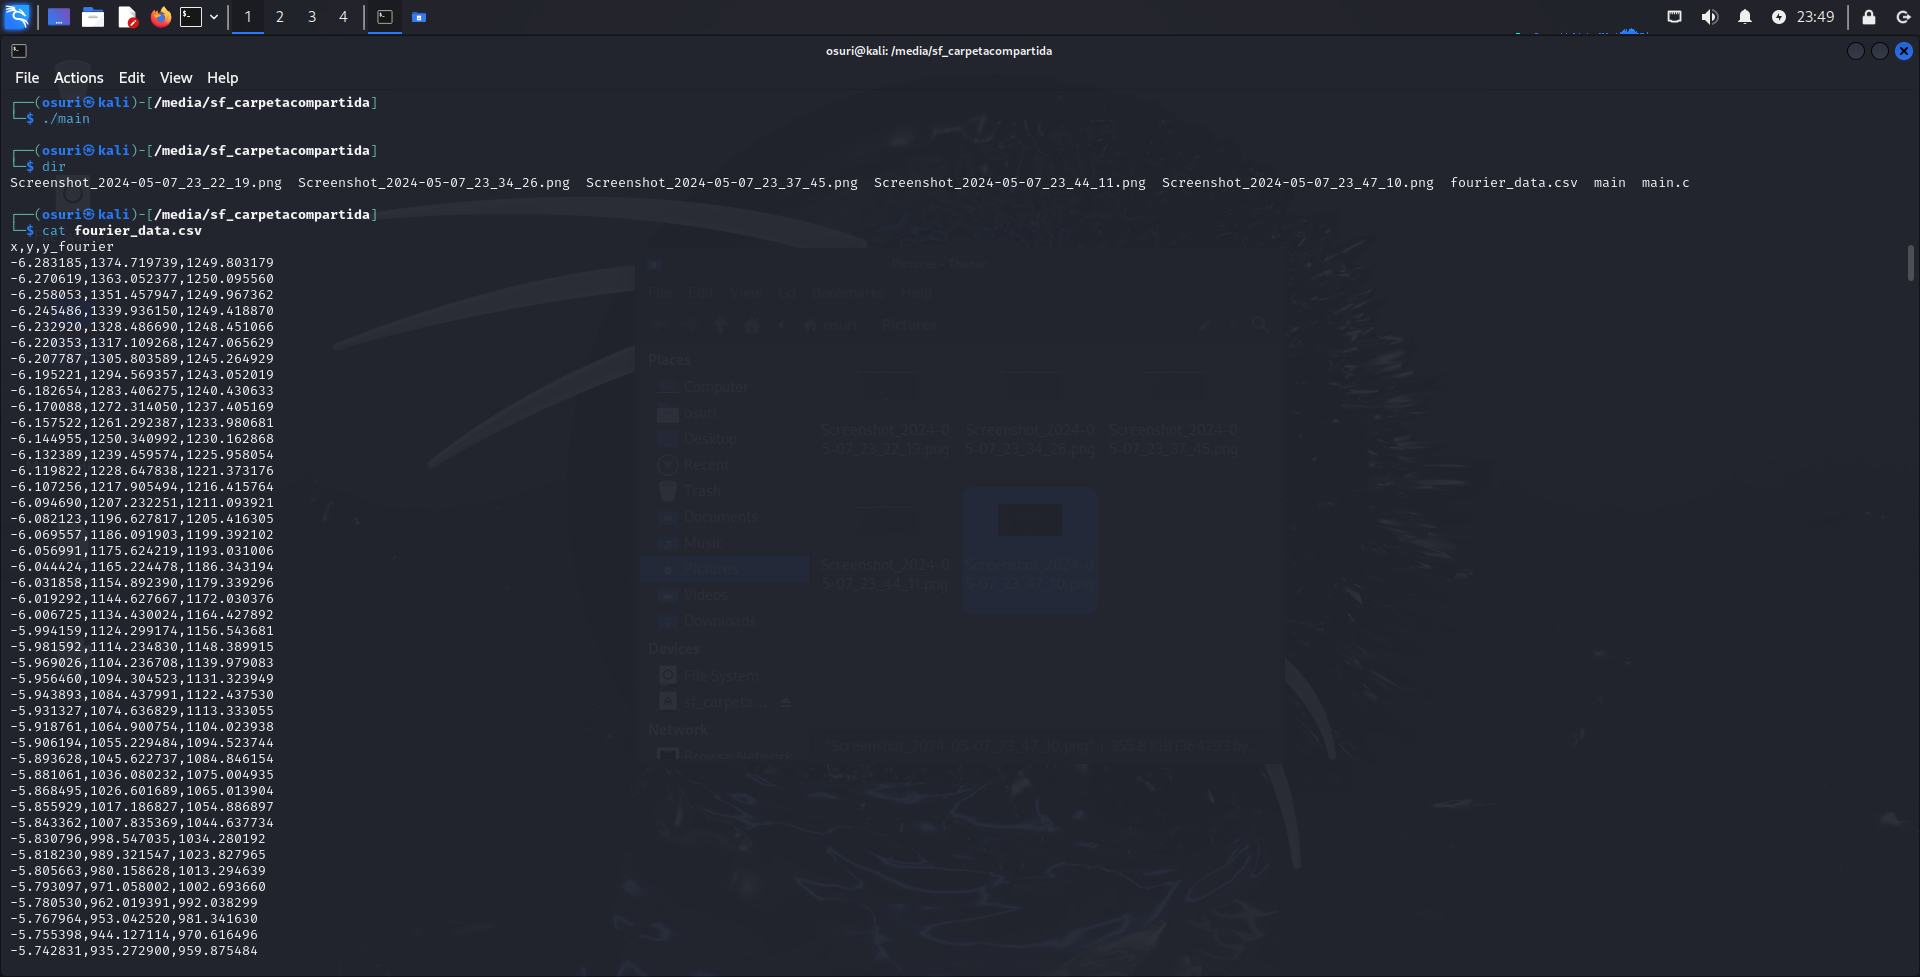
\includegraphics[width=2.29583in,height=4.29598in]{media/image35.png}

Imagen 20. Datos de archivo CSV. Fuente: Autoría propia

\begin{enumerate} \def\labelenumi{\arabic{enumi}.} \setcounter{enumi}{2} \item   Gráfica generada por este conjunto de datos (ver figura 5) \end{enumerate}

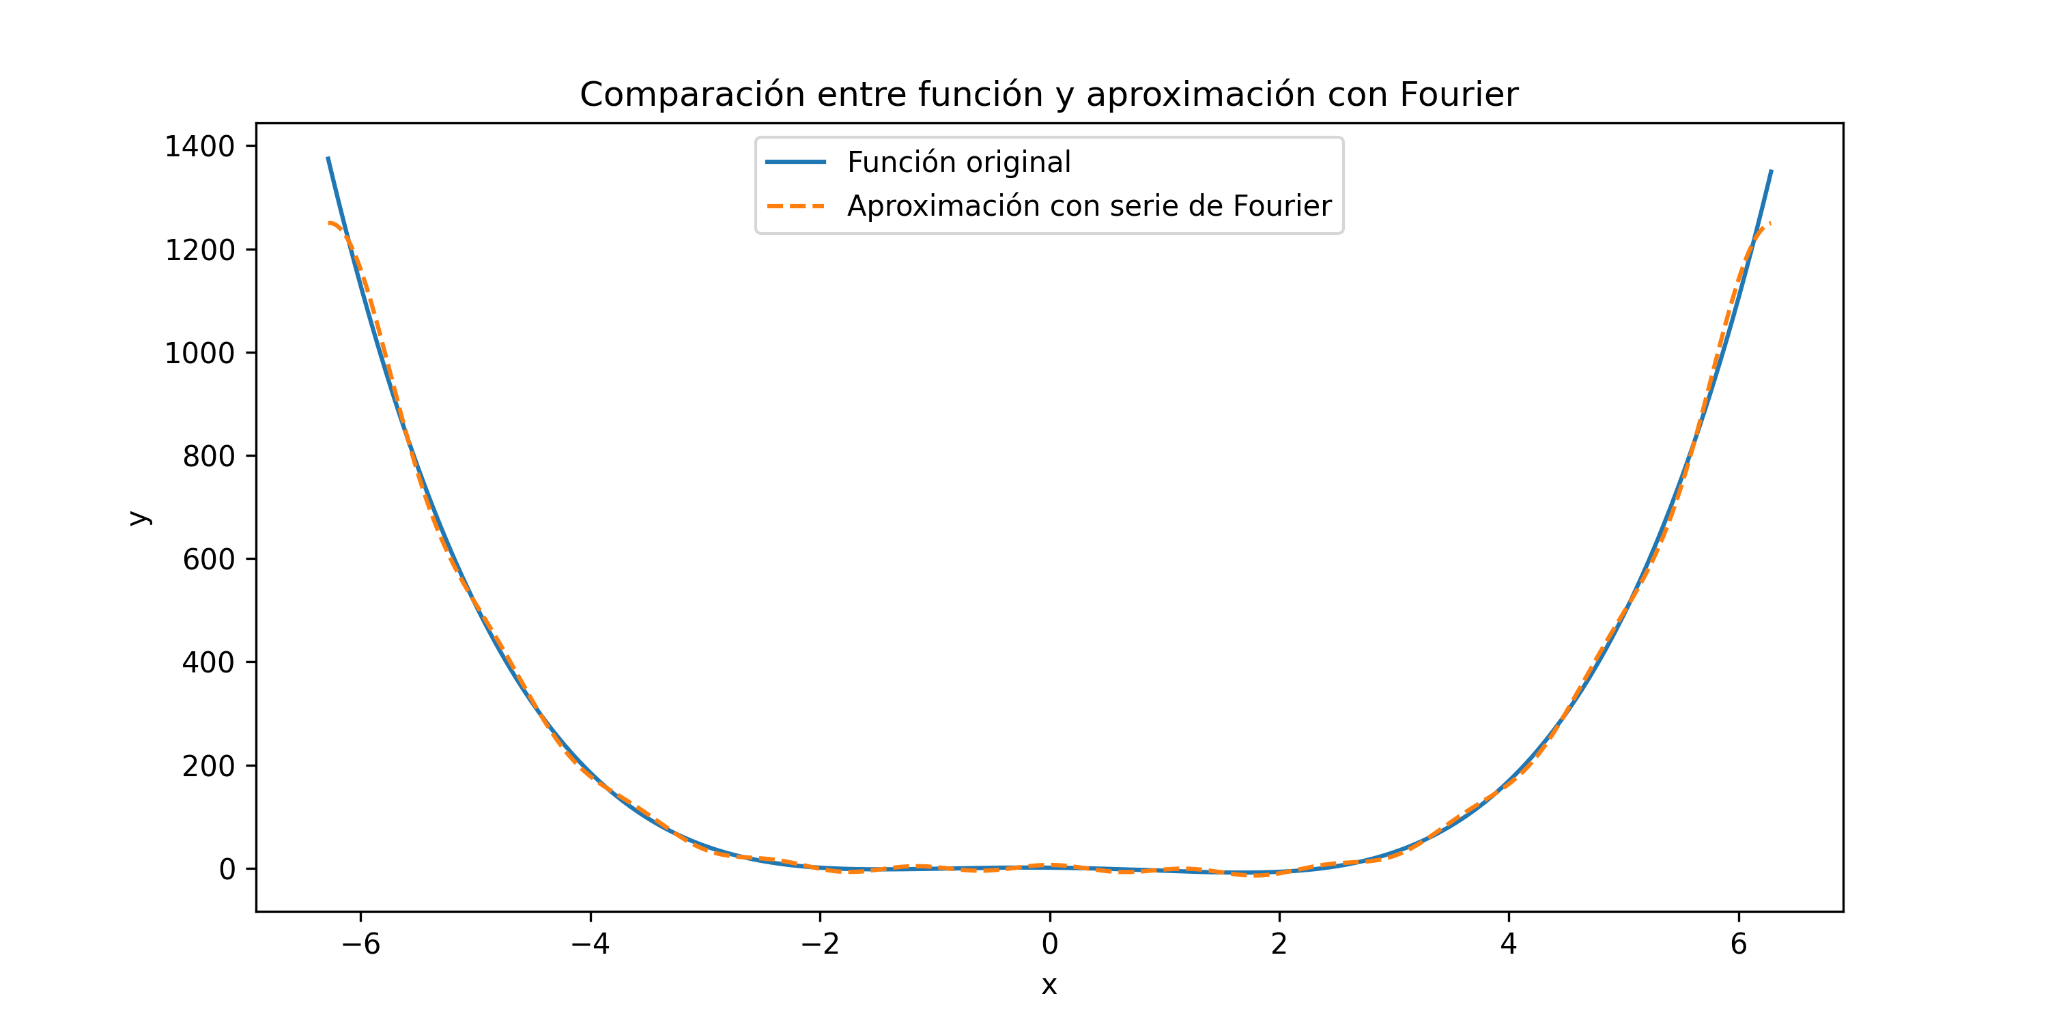
\includegraphics[width=6.26772in,height=3.13889in]{media/image30.png}

Figura 5. Gráfica generada. Fuente: Autoría propia
